\newpage
\thispagestyle{sectioned}
\chapter{Diseño de la Aplicación}

\section{Introducción}

Tras haber adaptado (Ver Sección \ref{sec:migration}) la tecnología de Wave/SwellRT a Android que soportaría el núcleo de nuestra aplicación, era hora de decidir qué aplicación le íbamos a dar de cara a desarrollar una aplicación Android que hiciera uso de ello. Era importante tener en cuenta las características que nos ofrecía Wave:

 - Edición colaborativa.

 - Consistencia en Tiempo Real.
 
\section{Brainstorming de ideas}  

Después de considerar posibles ideas de implementaciones que podrían hacer uso de estas características, decidimos realizar una sesión de \textit{brainstorming} junto a nuestros directores de proyecto para identificar ideas potenciales. En esta sesión aparecieron temas tan variados como wikis colaborativas, aplicaciones de inteligencia artificial, aportaciones colaborativas en política, edición de vídeos y música, cursos de formación colaborativos, visualizacion de mapas, etc.

	\begin{figure}[H]
        \centering
        \begin{subfigure}[b]{0.7\textwidth}
                \includegraphics[width=\textwidth]{Media/Captures/brainstorming.jpg}
                \caption{Idea de Aplicación}
                \label{fig:brainstormingApp}
        \end{subfigure}
        ~
        \begin{subfigure}[b]{0.7\textwidth}
                \includegraphics[width=\textwidth]{Media/Captures/appname.jpg}
                \caption{Posibles Nombres}
                \label{fig:brainstormingName}
        \end{subfigure}
        \caption{Capturas del brainstorming}\label{fig:brainstormingCaptures}
	\end{figure}
	


Con un gran repertorio de ideas expuestas en la sesión, decidimos centrarnos primero en descartar aquellas que a nosotros no nos motivaba llevar a cabo. De esta manera nos quedamos con cuatro ideas fundamentales a desarrollar en nuestra aplicación: Política, Música, Inteligencia Artificial y Mapas. Centrándonos ahora solo en estos temas, surgieron varias ideas colaborativas como: desarrollar documentos políticos, programas electorales, comunicación entre colectivos en tiempo real, aprendizaje de música, edición de partituras y obras, aplicaciones colaborativas con inteligencia artificial, edición de mapas en tiempo real, lexicalización, etc.

Finalmente, ya que ambos teníamos interes por la política, decidimos realizar una aplicación colaborativa relacionada con dicho mundo. En esta aplicación podríamos recurrir a la edición de contenidos en tiempo real, ya fueran propuestas políticas, programas electorales u otro tipo de documentos. Más adelante también podríamos hacer uso incluso de alguna herramienta de Inteligencia Artificial para automatizar algunas tareas o realizar recomendaciones sociales.

Lo que sí que tuvimos claro desde el principio es la idoneidad del momento actual para desarrollar una aplicación de temática política, dado que nos encontramos en año electoral. Nos propusimos el objetivo de desarrollar algo que pudiera tener cierta repercusión y utilidad en las próximas citas electorales de este año 2015. Intentariamos pensar en la aplicación no solo como un Trabajo de Fin de Grado sino como algo que pudiéramos llevar más allá y que resultara útil a la sociedad.

Por otro lado, queriamos elegir un nombre para la aplicación que fuera a la vez atractivo y significativo de la participación ciudadana que representa. Para esto hicimos tambien una sesión de \textit{brainstorming} con varias personas, de la cual sacamos varias posibilidades por el nombre. Tras someter a votación estos nombres nos quedamos con el que más gustó a todos: \textbf{DemoCritics}.

\section{Diseño Guiado Por Objetivos (DGO)}

En este capítulo se desarrollan las fases de la metodología del Diseño Guiado por Objetivos (ver sección \ref{ssec:dgoDesign}). Cada una de ellas especificará los pasos a seguir durante su progreso y el resultado final de cada una.

\subsection{Investigación}

\subsubsection{Intención Inicial: Prototipo básico}  

Vivimos en una época donde la política parece estar de moda. Esto puede ser debido al cabreo general que muestra la ciudadanía frente a gobiernos conservadores, situaciones de austeridad provocada por la crisis económica, el nacimiento de nuevas fuerzas políticas, …, pero sobre todo las numerosas citas electorales a las que seremos citados en 2015. Por tanto, el proyecto podría ponerse a prueba en un escenario real durante la campaña de las elecciones generales previsiblemente convocadas durante el último trimestre del 2015.

\underline{Programas electorales}

La intención fundamental de la aplicación es llevar los programas electorales a los bolsillos de los ciudadanos y generar interés en participar más activamente en la política, ya sea emitiendo opiniones sobre dichos programas o elaborando nuevas propuestas. Vivimos en una sociedad digital, donde cada vez son más las personas que utilizan sus smartphones para realizar todo tipo de tareas en su vida cotidiana.

En los últimos años las diferentes formaciones políticas han subido sus programas electorales a un documento en formato PDF que suele estar disponible para su descarga en su página web. Este documento tiene generalmente una gran extensión (los hay de 200 páginas), lo cual no hace sino dificultar que las personas se animen a leerlo. Por ello pensamos que una aplicación que pudiera visualizar las principales secciones de los programas políticos podría ser especialmente útil para acercar los programas a los electores.

Además también intentariamos darle una estructura a estos programas, de manera que el usuario pudiera navegar por ellos a nivel de Sección, a diferencia del método actual de leer un "macro-documento" en PDF. Así, la gente podría opinar sobre los programas políticos a nivel de sección mediante acciones familiares para ellos: "Me gusta", "No me gusta" y realizar "Comentarios". Añadimos también una acción de "No lo entiendo" que pensamos que seria util para indicar cuándo la redacción de la sección era de significado difuso.

En definitiva, queríamos crear un espacio donde poder informarse sobre las distintas ofertas electorales y poder debatir sobre las propuestas que propone cada formación política, todo ello en forma una aplicación que podremos consultar en cualquier momento. 

\underline{Propuestas y Wave}

Por otro lado,y en línea con los últimos movimientos políticos ciudadanos, pretendíamos crear también un portal de propuestas ciudadanas en el móvil. Los usuarios podrían visualizar las propuestas de otros usuarios y tener la posibilidad de crear nuevas propuestas. Además, como queríamos aprovechar las características de la migración de Wave previamente desarrollada, pensamos en la posibilidad de elaborar estas propuestas de forma colaborativa y en tiempo real entre muchos usuarios.

Actualmente existen multitud de portales (en su gran mayoría web) donde la ciudadanía puede expresar su opinión, pero creemos que la integración de una aplicación donde puedan situarse las opiniones de los partidos políticos (en forma de sus programas) y la actividad ciudadana (en forma de propuestas), genera una nueva manera de tratar la política en los medios sociales.

También pensamos en la posibilidad de categorizar el contenido de la aplicación (Programas y Propuestas) por temas, para proporcionar filtros a la hora de navegar por dicho contenido. Sin embargo no teníamos muy clara la elección de temas, asi como si debiamos darle al usuario la posibilidad de crear nuevos temas o dar nosotros unos temas preestablecidos.
 
Una vez pensada la intención y los principales objetivos de la aplicación, procedimos a realizar unos primeros prototipos en papel de nuestra idea y a implementar un prototipo básico en el móvil (Ver Sección \ref{ssec:prototypes}) que mostraba programas políticos estructurados y permitía navegar a nivel de Sección por ellos para leer y emitir opiniones (likes, dislikes, comentarios, etcétera.).  

\subsubsection{Hipótesis de personas}

Para identificar a los usuarios objetivo, tenemos que encontrar a miembros representativos de esos usuarios y animarlos a que participen en nuestra investigación. Para ello reuniremos una serie de características básicas que el usuario deberá cumplir para poder aportarnos los objetivos funcionales de la aplicación. Estas son algunas de las caracaerísticas deseadas:

\begin{itemize}
\item \textbf{Edad}: Entre 16 y 65 años.
\item \textbf{Sexo}: Indiferente.
\item \textbf{Profesión}: Indiferente.
\item \textbf{Aptidudes deseables}: Activismo social, cociencia política, trabajo colaborativo, ... .
\item \textbf{Habilidades técnicas}: Usuario con experiencia media en uso de aplicaciones móviles.
\end{itemize}

Simplificando el tipo de persona que queremos encontrar, lo dividiremos en dos tipos de persona. Por un lado buscaremos al activista social, activo en movimientos sociales, participación en portales con carácter social, etcétera. Mientras que por otro lado buscaremos una persona que muestre cierto interés en el mundo de la política, pero que no participe en moviimentos sociales. Finalmente pudimos contactar con dos miembros de Labodemo \cite{ref:labodemo}, una organización que se dedica al desarollo de nuevas formas de participación ciudadana. Este perfil cubiría en caso del activista social, mientras que para el tipo de persona entendido de la política pero no tan involucrado, escogimos a Javier de la Cueva \cite{ref:jdelacueva}.

El siguiente paso sería estudiar la viabilidad de esta aplicación entrevistando a las personas seleccionadas para realizar una investigación sobre sus necesidades prácticas. Por otra parte también sería útil enseñarles los prototipos básicos que manejábamos para verificarlos. Entendimos que el tipo de persona con el que nos entrevistáramos debía de estar relacionado de alguna manera con el mundo de la política, pues nada mejor que hablar con gente ya interesada en dichos temas para orientarnos por el buen camino.

A continuación detallamos las entrevistas que realizamos en la investigación:

\subsubsection{Entrevista con Labodemo}

Tuvimos la oportunidad de mantener una conversación con dos miembros de Labodemo \cite{ref:labodemo}, en la que aprovechamos para mostrarles un prototipo de la aplicación que estábamos desarrollando. Ambos tenían experiencia en el desarrollo de plataformas de participación ciudadana en Internet: fueron los responsables del desarrollo de los portales de participación del partido político Podemos y la candidatura ciudadana de unidad popular Ahora Madrid.

En ese momento nuestro prototipo móvil se limitaba únicamente a mostrar las diferentes secciones de cada programa, lo cual les pareció útil, aunque no lo suficiente como para atraer a una cantidad considerable de usuarios. Conforme a su linea de trabajo habitual, eran más partidarios de dar a los usuarios la posibilidad de realizar Propuestas además de ver Programas políticos. Les comentamos entonces que antes de hablar con ellos ya habíamos planteado desarrollar Propuestas colaborativas en tiempo real aprovechando la tecnología de Wave. Pero ellos no eran partidarios de esta opción, ya que según ellos acabaría siendo caótico tener tanta gente editando la misma propuesta de cara a generar contenido útil. 

Dándole una vuelta a la categorización del contenido, nos sugirieron que para atraer a usuarios, debíamos considerar la posibilidad de integrar en la aplicación a colectivos sociales que generaran y categorizaran dicho contenido. No eran partidarios de que dieramos nosotros ciertas temáticas preestablecidas, pues debido a la variedad de redaccion en los distintos programas sería dificil identificar temáticas que incluyeran a todos los programas y probablemente acabariamos excluyendo temas. Así, serían los colectivos los que se encargaran de "tematizar" el contenido de la aplicación. Por ejemplo: un grupo de animalistas podría tener un espacio en la aplicación donde poder crear sus propias propuestas, e incluso hacer comparativas de lo que proponen los diferentes programas sobre los animales. 

De esta manera, y en relación a la aproximación a los foros tradicionales, se planteó la idea de crear "Hilos": elementos "temáticos" que agruparan en un solo sitio Secciones y Propuestas que hablaran sobre un determinado tema. Estos hilos serían también generados por dichos colectivos.

Esto sería útil también para usuarios que buscaran información sobre un determinado tema. Por ejemplo: un usuario poco activo, que resulta ser profesor, podría buscar un colectivo de profesores y ver las Propuestas que se llevan a cabo o visualizar una comparativa respecto las medidas de educación de los diferentes programas políticos.

Nos insistieron mucho en el tema de las comparativas. Sería de gran utilidad que la aplicación tuviera una parte de comparativas en la que los usuarios pudieran comparar los programas políticos en vez de leerlos sección por sección. Resultaría de gran interés a un autónomo visualizar las medidas que proponen los diferentes partidos políticos para los autónomos. Pero estas comparativas no podría realizarlas cualquiera, por lo que deberían realizarlas periodistas o expertos que hubieran realizado algún tipo de comparativa similar anteriormente. Nos sugirieron contactar con periodistas o colectivos que hubieran publicado algún tipo de comparativa en cuanto a programas o medidas, para obtener algún tipo de ayuda o consejo a seguir.

\subsubsection{Conclusión}

\underline{Puntos positivos}:

\begin{itemize}
 \item Nueva forma de participación ciudadana de cara a las elecciones.
 \item Métodos alternativos para discutir propuestas, partidos, programas, etcétera.
 \item Ligar propuestas a programas concretos.
\end{itemize}

\underline{Puntos negativos}:

\begin{itemize}
 \item Visualizar un programa electoral en el móvil puede no resultar demasiado interés para los usuarios.
 \item Desarrollar propuestas colaborativas en tiempo real no maniene una estabilidad en la aplicación.
 \item La aplcación debería desarrollarse en otras plataformas móviles y de escritorio.
\end{itemize}

\underline{Puntos a tener en cuenta}:

\begin{itemize}
 \item Dejar libertad a usuarios y colectivos creando sus propias categorías o hilos como ''Espacios'' que puedan elaborar segun sus intereses y generar contenido para la aplicación.
 \item Desarrollar comparativas por secciones, temas o partidos. De tal forma que un usuario pueda visualizar las diferencias de aquellos temas que le preocupan.
 \item Contactar con colectivos, asociaciones y/o periodistas que anteriormente hayan elaborado comparativas entre programas políticos en puntos concretos
\end{itemize}

\subsubsection{Entrevista con Javier de la Cueva}

La entrevista con Javier de la Cueva resultó bastante productiva. Ya le conocíamos de algunas conferencias que impartió en la facultad. Javier es abogado y doctorado en Filosofía, estando especializado en temas relacionados con tecnología, Internet y propiedad intelectual. Además, en sus últimas conferencias Javier habla sobre acciones micropolíticas \cite{ref:manualCiberactivista}. Estas acciones definen la capacidad que tienen los ciudadanos para realizar aportaciones a la sociedad, el estado o el gobierno que favorezcan la participación ciudadana en una democracia participativa.

Representar los programas electorales en una aplicación móvil le pareció algo interesante y necesario para la sociedad actual. Si bien casi nadie hace el esfuerzo de visualizar un programa electoral en PDF, utilizar una herramienta que facilita el acceso al programa por secciones podría ser una nueva forma de incentivar su lectura y ayudar a fomentar la participación ciudadana en política. 

Además nos sugirió la posibilidad de desarrollar una Hemeroteca de programas electorales. De esta forma cualquiera podría consultar los programas de los anteriores gobiernos y comprobar si se cumplieron los objetivos del programa, así como comparar programas de distintos años entre sí, 

Pero si en algo nos insistió Javier, fue en la importancia de categorizar el contenido de la aplicación. Un usuario que no tenga conocimientos sobre diversos temas, se encontraría más cómodo si pudiera visualizar las diferentes partes de un programa o las propuestas ciudadanas por categorías o temas generales. Ya que dejar libertad a los usuarios para crear categorías personalizadas podría ser algo negativo para usuarios inexpertos o con pocos conocimientos sobre temas específicos.

Por último, centrándonos en las Propuestas ciudadanas, surgió la idea de elaborar propuestas que tuvieran una especificación concreta. Es decir, a parte de tener una idea de propuesta y redactarla, esta propuesta debería ir acompañada de los recursos que serían necesarios y sobre todo cómo se llevaría a cabo de una forma aproximada. También resultaría interesante definir un pequeño presupuesto de lo que conllevaría realizar la propuesta o cómo se podría financiar. Así evitaríamos una elaboración de propuestas más real, evitando un listado de propuestas infinito sin planterase cómo se llevarían a cabo o cómo se financiarían.

\subsubsection{Conclusión}

\underline{Puntos positivos}:

\begin{itemize}
  \item Llevar los programas políticos de una forma más atractiva a la ciudadanía es algo esencial en la actualidad.
  \item Categorizar las secciones de los programas políticos para que se puedan explorar por temas.
  \item Incluir los recursos necesarios que hacen falta para llevar una propuesta a cabo.
\end{itemize}

\underline{Puntos negativos}:

\begin{itemize}
  \item Tratar de convertir la aplicación en un \textit{foro} inconscientemente.
  \item Dejar libertad a la hora de crear categorías específicas o hilos puede generar confusión entre los usuarios. 
\end{itemize}

\underline{Puntos a tener en cuenta}:

\begin{itemize}
  \item Desarrollar categorías semanales en función de las novedades o actualidad política.
  \item Añadir la posibilidad de solicitar la ayuda de expertos sobre un tema para elaborar una propuesta.
  \item Crear una emeroteca de programas políticos para realizar análisis sobre el cumplimiento de los programas en legislaturas pasadas.
  \item Informar sobre la legilación actual cuando visualicemos una propuesta o sección de un porgrama que quiera mejorar o cambiar la legislación actual.
\end{itemize}

\subsection{Modelado de Personas}

Las \textit{personas} son una herramienta de diseño y ayuda al diseño de la aplicación. El objetivo es centrar el diseño en este tipo de persona, para lograr los objetivos a la hora de utilziar un sistema. La \textit{persona} será nuestro modelo, una descripción detallada de un individuo imaginario que representa a un grupo de usuarios a los que va destinada la aplicación. Es una representación ficticia pero desarrollada con gran detalle, que será fruto de los datos recogidos en la investigación previa de la fase anterior.

En esta fase definiremos el tipo de persona que interactuará con nuestra aplicación. Para ello hemos identificado dos tipos de personas primarias; un \textbf{activista social} y un \textbf{ciudadano} de a pie que forme parte del electorado.

\textbf{- Activista social, 16 años en adelante}

\underline{Actividad:}

\begin{itemize}
\item Estudia, trabaja o realiza otras actividades de voluntariado.
\item Frecuenta asambleas, participa en diferentes movimientos sociales y está al día de la actualidad política.
\item Utiliza redes sociales para comunicarse con otros colectivos, acudir a asambleas, promover ideas u otras actividades relacionadas con la política y el activismo social.
\end{itemize}

\underline{Otros:}

\begin{itemize}
\item Desconoce las ideas que proponen algunos partidos 
\item Le gusta aportar nuevas soluciones a la sociedad.
\end{itemize}

\textbf{- Ciudadano de a pie, 18 años en adelante}

\underline{Actividad:}

\begin{itemize}
\item Estudia, trabaja o realiza otras actividades de voluntariado.
\item Es distante al mundo de la política, concibe ciertos temas pero no los conoce en profundidad.
\item Visita diferentes medios de comunicación para enterase de la actualidad.
\item Utiliza redes sociales para compartir contenidos con sus amigos o establecer nuevas amistades.
\end{itemize}

\underline{Otros:}

\begin{itemize}
\item Desconoce por completo los programas electorales. 
\item Tiene cierta indecisión a la hora de acudir a las urnas, no sabe que propone cada partido.
\end{itemize}

\subsection{Definición de personas}

En las figuras \ref{fig:studentPerson} y \ref{fig:activistPerson} se exponen una serie de personas ficticias que podrían representar en la vida real los tipos de \textit{persona} a la que va dirigida la aplicación.

	\begin{figure}[!]
      \centering
	\includegraphics[keepaspectratio, scale=0.45]{Media/Captures/person1.png}
      \caption{Estudiante universitario}
      \label{fig:studentPerson}
    \end{figure}
    
	\begin{figure}[!]
      \centering
	\includegraphics[keepaspectratio, scale=0.45]{Media/Captures/person2.png}
      \caption{Activista político}
      \label{fig:activistPerson}
    \end{figure}


\subsection{Definición de Escenarios y Requisitos}

En esta sección se definirán los posibles escenarios que puedan surgir en la aplicación. La idea es situarnos en un escenario real que pudera ocurrir en cualquier momento a lo largo del día, para detallar la solución al problema. En cada uno se especificarán los requisitos necesarios para solventar el problema o los pasos a seguir para lograr el objetivo. Diferenciaremos los términos de \textbf{acción}, como la actividad inmediata que requiere la solución. El \textbf{objeto}, como el sujeto principal del escenario. Y por último definimos \textbf{contexto} reflejando el objetivo final del requisito.

\textbf{Escenario I}

Se acercan las elecciones municipales y Juan aún no ha decidido a qué partido va dar su voto. No conoce las propuestas que ofertan los partidos a la ciudadanía y tampoco se fía mucho de lo que dicen los medios de comunicación.

Juan coge su móvil y visualiza los diferentes programas electorales por categoría, seleccionando la categoría de educación que es la que más le afecta a él personalmente. La aplicación le muestra un listado de las secciones donde lso diferentes partidos hablan de las medidas que van a tomar en torno a la educación.

\underline{Requisitos:}

\begin{enumerate}
\item Visualizar (acción) las diferentes categorías (objeto), para ver las secciones de los programas de una determinada categoría (contexto).
\item Mostrar(acción) un listado de todas las secciones de los programas de los partidos  políticos (objeto) en función de la categoría seleccionada por el usuario (contexto).
\end{enumerate}

\textbf{Escenario II}

Pablo es un empleado sanitario de Hospital Clínico de Madrid preocupado por la gestión de los hospitales públicos. Parece que la situación no está muy controlada, por lo que quisiera saber que propuestas o alternativas propone la ciudadanía para mejorar la situación actual.

A través de su móvil puede explorar las diferentes propuestas por categorías. Eligiendo la categoría de sanidad, le aparece un listado de las últimas propuestas desarrolladas por la ciudadanía.

\underline{Requisitos:}

\begin{enumerate}
\item Visualizar (acción) el listado de propuestas (objeto), clasificados por la categoría seleccionada por el usuario (contexto).
\item Mostrar (acción) la propuesta (objeto), seleccionada por el usuario para que pueda puntuarla y/o comentarla (contexto).
\end{enumerate}

\textbf{Escenario III}

Lara es una profesora de un colegio de la Comunidad de Madrid. Se acercan las vacaciones de verano y muchos niños se quedarán sin acceso a comedor. Lara está planteándose cómo elaborar una propuesta ciudana para abrir los colegios en horario no lectivo y que todos los niños tengan derecho a comedor en los meses de verano. Lara no es una experta en gestión pública ni sabe cómo llevar a cabo la propuesta.

Para ello, Laura comienza a desarrollar una propuesta ciudadana en la aplicación, explicando la base de la propuesta. Al no saber cómo financiarlo, deja la propuesta abierta para que la comunidad la pueda ayudar a desarrollarla.

\underline{Requisitos:}
\begin{enumerate}
\item Agregar (acción) una nueva propuesta (objeto) rellenando los principales campos del formulario (contexto).
\item Publicar (acción) la propuesta (objeto) como una propuesta colaborativa para editar (contexto)
\item Mostrar (acción) la propuesta (contexto) en la lista de propuestas colaborativas para que puedan colaborar otros usuarios (contexto).
\end{enumerate}

\textbf{Escenario IV}

Fran es un periodista de un periódico digital. Se acercan las elecciones y está redactando un pequeño artículo acerca de los programas de algunos partidos políticos. Necesita acceder a los programas compeletos de los partidos y visualizar las secciones que le resulten de interés para comentarlas en su artículo.

Accediendo a la aplicación, Fran puede seleccionar los programas de todos los partidos que se presentan a las elecciones. Listando el índice del programa y accediendo a sus secciones.

\underline{Requisitos:}

\begin{enumerate}
\item Visualizar (acción) todos los partidos (objeto) que se presentan a las elecciones (contexto).
\item Seleccionar (acción) un partido polítco (objeto) para visualizar el programa electoral (contexto).
\item Listar (acción) el índice (objeto) de secciones del programa seleccionado (contexto).
\item Visualizar (acción) la sección (objeto) del programa seleccionado por el usuario (contexto).
\end{enumerate}

\subsection{Framework de diseño} \label{ssec:prototypes}

En esta sección detallaremos todos los aspectos relacionados con el desarrollo del aspecto visual y la interacción con la aplicación. Se utilizarán los escenarios y requisitos definidos en la fase anterior para crear los bocetos y prototipos interactivos. Detallaremos los prototipos desarrollados en papel, algunos prototipos intermedios y el prototipo final de la aplicación presentado.

\subsubsection{Framework de interacción}

Para definir el Framework de interacción realizaremos un proceso de seis etapas:

\textbf{Factor de forma, postura y métodos de entrada}

La aplicación será visualizada en un smartphone bajo el sistema operativo Android (con API 15 como mínimo), con tamaños de pantalla entre 3,5 y 6 pulgadas. Que pueda visualizarse en interiores y exteriores.

La \textbf{postura} será \textbf{temporal}. El usuario puede utilizarlo en periodos de tiempo muy breves como puede ser la consulta de alguna sección, propuesta o dar su valoración. Elaborando una propuesta o participando en el desarrollo de una, el usuario necesitará algo más de tiempo, pero seguirá utilizando funciones básicas. Propias de una postura temporal. \\[2cm.]

\textbf{Elementos y datos funcionales} 

\underline{Elementos de datos}:

\begin{itemize}
 \item Programa político
 \begin{itemize}
  \item \underline{Atributos}: partido, programa, secciones, índice, temas.
  \item \underline{Relaciones}: partido-programa, índice-sección.
 \end{itemize}
\end{itemize}

\begin{itemize}
 \item Temas
 \begin{itemize}
  \item \underline{Atributos}: categoría, programa, sección, partido, propuesta.
  \item \underline{Relaciones}: categoría-programa, categoría-propuesta, partido-sección.
 \end{itemize}
\end{itemize}

\begin{itemize}
 \item Propuestas Ciudadanas
 \begin{itemize}
  \item \underline{Atributos}: propuesta, categoría, usuario.
  \item \underline{Relaciones}: propuesta-usuario, propuesta-categoría.
 \end{itemize}
\end{itemize}

\begin{itemize}
 \item Propuestas Colaborativas
 \begin{itemize}
  \item \underline{Atributos}: propuesta, categoría, usuario, edición colaborativa.
  \item \underline{Relaciones}:  usuario-propuesta, propuesta-categoría.
 \end{itemize}
\end{itemize}

\underline{Elementos funcionales}:

 \begin{itemize}
  \item Visualizar los partidos políticos que se presentan a las elecciones.
  \item Mostrar el índice de cada programa político.
  \item Mostrar, valorar y debatir las secciones de los programas políticos.
  \item Visualizar categorías por temas, distinguiendo entre propuestas y secciones de programas.
  \item Mostrar, valorar y debatir las propuestas de los usuarios.
  \item Crear una nueva propuesta en una categoría.
  \item Mostrar las propuestas colaborativas y participar en su desarrollo.
  \item Crear una nueva propuesta incompleta para desarrollarla de forma colaborativa.
 \end{itemize}

\textbf{Grupos funcionales y jerarquías}

Pantalla principal de la aplicación. Grupos de elementos funcionales que contiene:

\begin{itemize}
 \item Lectura y valoración de Programas políticos.
 \begin{itemize}
  \item Visualizar programas políticos.
  \item Ver secciones de programas.
  \item Visualización, valoración y debate de secciones de programas políticos.
 \end{itemize}
\end{itemize}

\begin{itemize}
 \item Clasificación de secciones de programas y propuestas ciudadanas por categorías.
 \begin{itemize}
  \item Ver secciones de programas políticos por tema.
  \item Ver propuestas ciudadanas por tema.
 \end{itemize}
\end{itemize}

\begin{itemize}
 \item Lectura, valoración y creación de Propuestas Ciudadanas.
 \begin{itemize}
  \item Ver propuestas ciudadanas.
  \item Valorar y debatir propuestas ciudadanas.
  \item Creación de propuesta ciudadana.
 \end{itemize}
\end{itemize}

\begin{itemize}
 \item Lectura, colaboración y creación de Propuestas Colaborativas.
 \begin{itemize}
  \item Visualizar las propuestas ciudadanas en desarrollo.
  \item Crear una propuesta colaborativa.
  \item Colaborar en el desarrollo de una propuesta.
 \end{itemize}
\end{itemize}

\textbf{Boceto del framework de interacción}

El proceso de desarrollo de bocetos se ha realizado en espiral, de tal forma que una vez que identificábamos una determinada funcionalidad, la representábamos en un mockup a papel para debatirlo y discutirlo en las entrevistas. A continuación trasladábamos el mockup a un prototipo de alto nivel desarrollado en Android. Para las siguientes implementaciones que añadían nueva funcionalidad el proceso era el mismo:

\begin{enumerate}
 \item Desarrollo de un boceto a papel identificando los elementos funcionales.
 \item Definir la interacción a través de la herramienta POP \cite{ref:pop}.
 \item Implementar un prototipo de mayor fidelidad en Android. 
\end{enumerate}

  \begin{figure}[h]
   \centering
	\includegraphics[keepaspectratio, scale=1]{Media/Captures/prototypesDiagram.png}
    \caption{Modelo de desarrollo de los prototipos.}
   \label{fig:sequenceDiagram_waveWebSocket}
  \end{figure}
  
De esta forma tuvimos que dar un total de tres vueltas a nuestro modelo en espiral para completar el desarrollo.

\begin{enumerate}
 \item \textbf{Programas Políticos}
 
 Estos fueron los primeros bocetos que definían la interacción de la visualización de los programas políticos:
 
 	\begin{figure}[H]
        \centering
        \begin{subfigure}[b]{0.3\textwidth}
                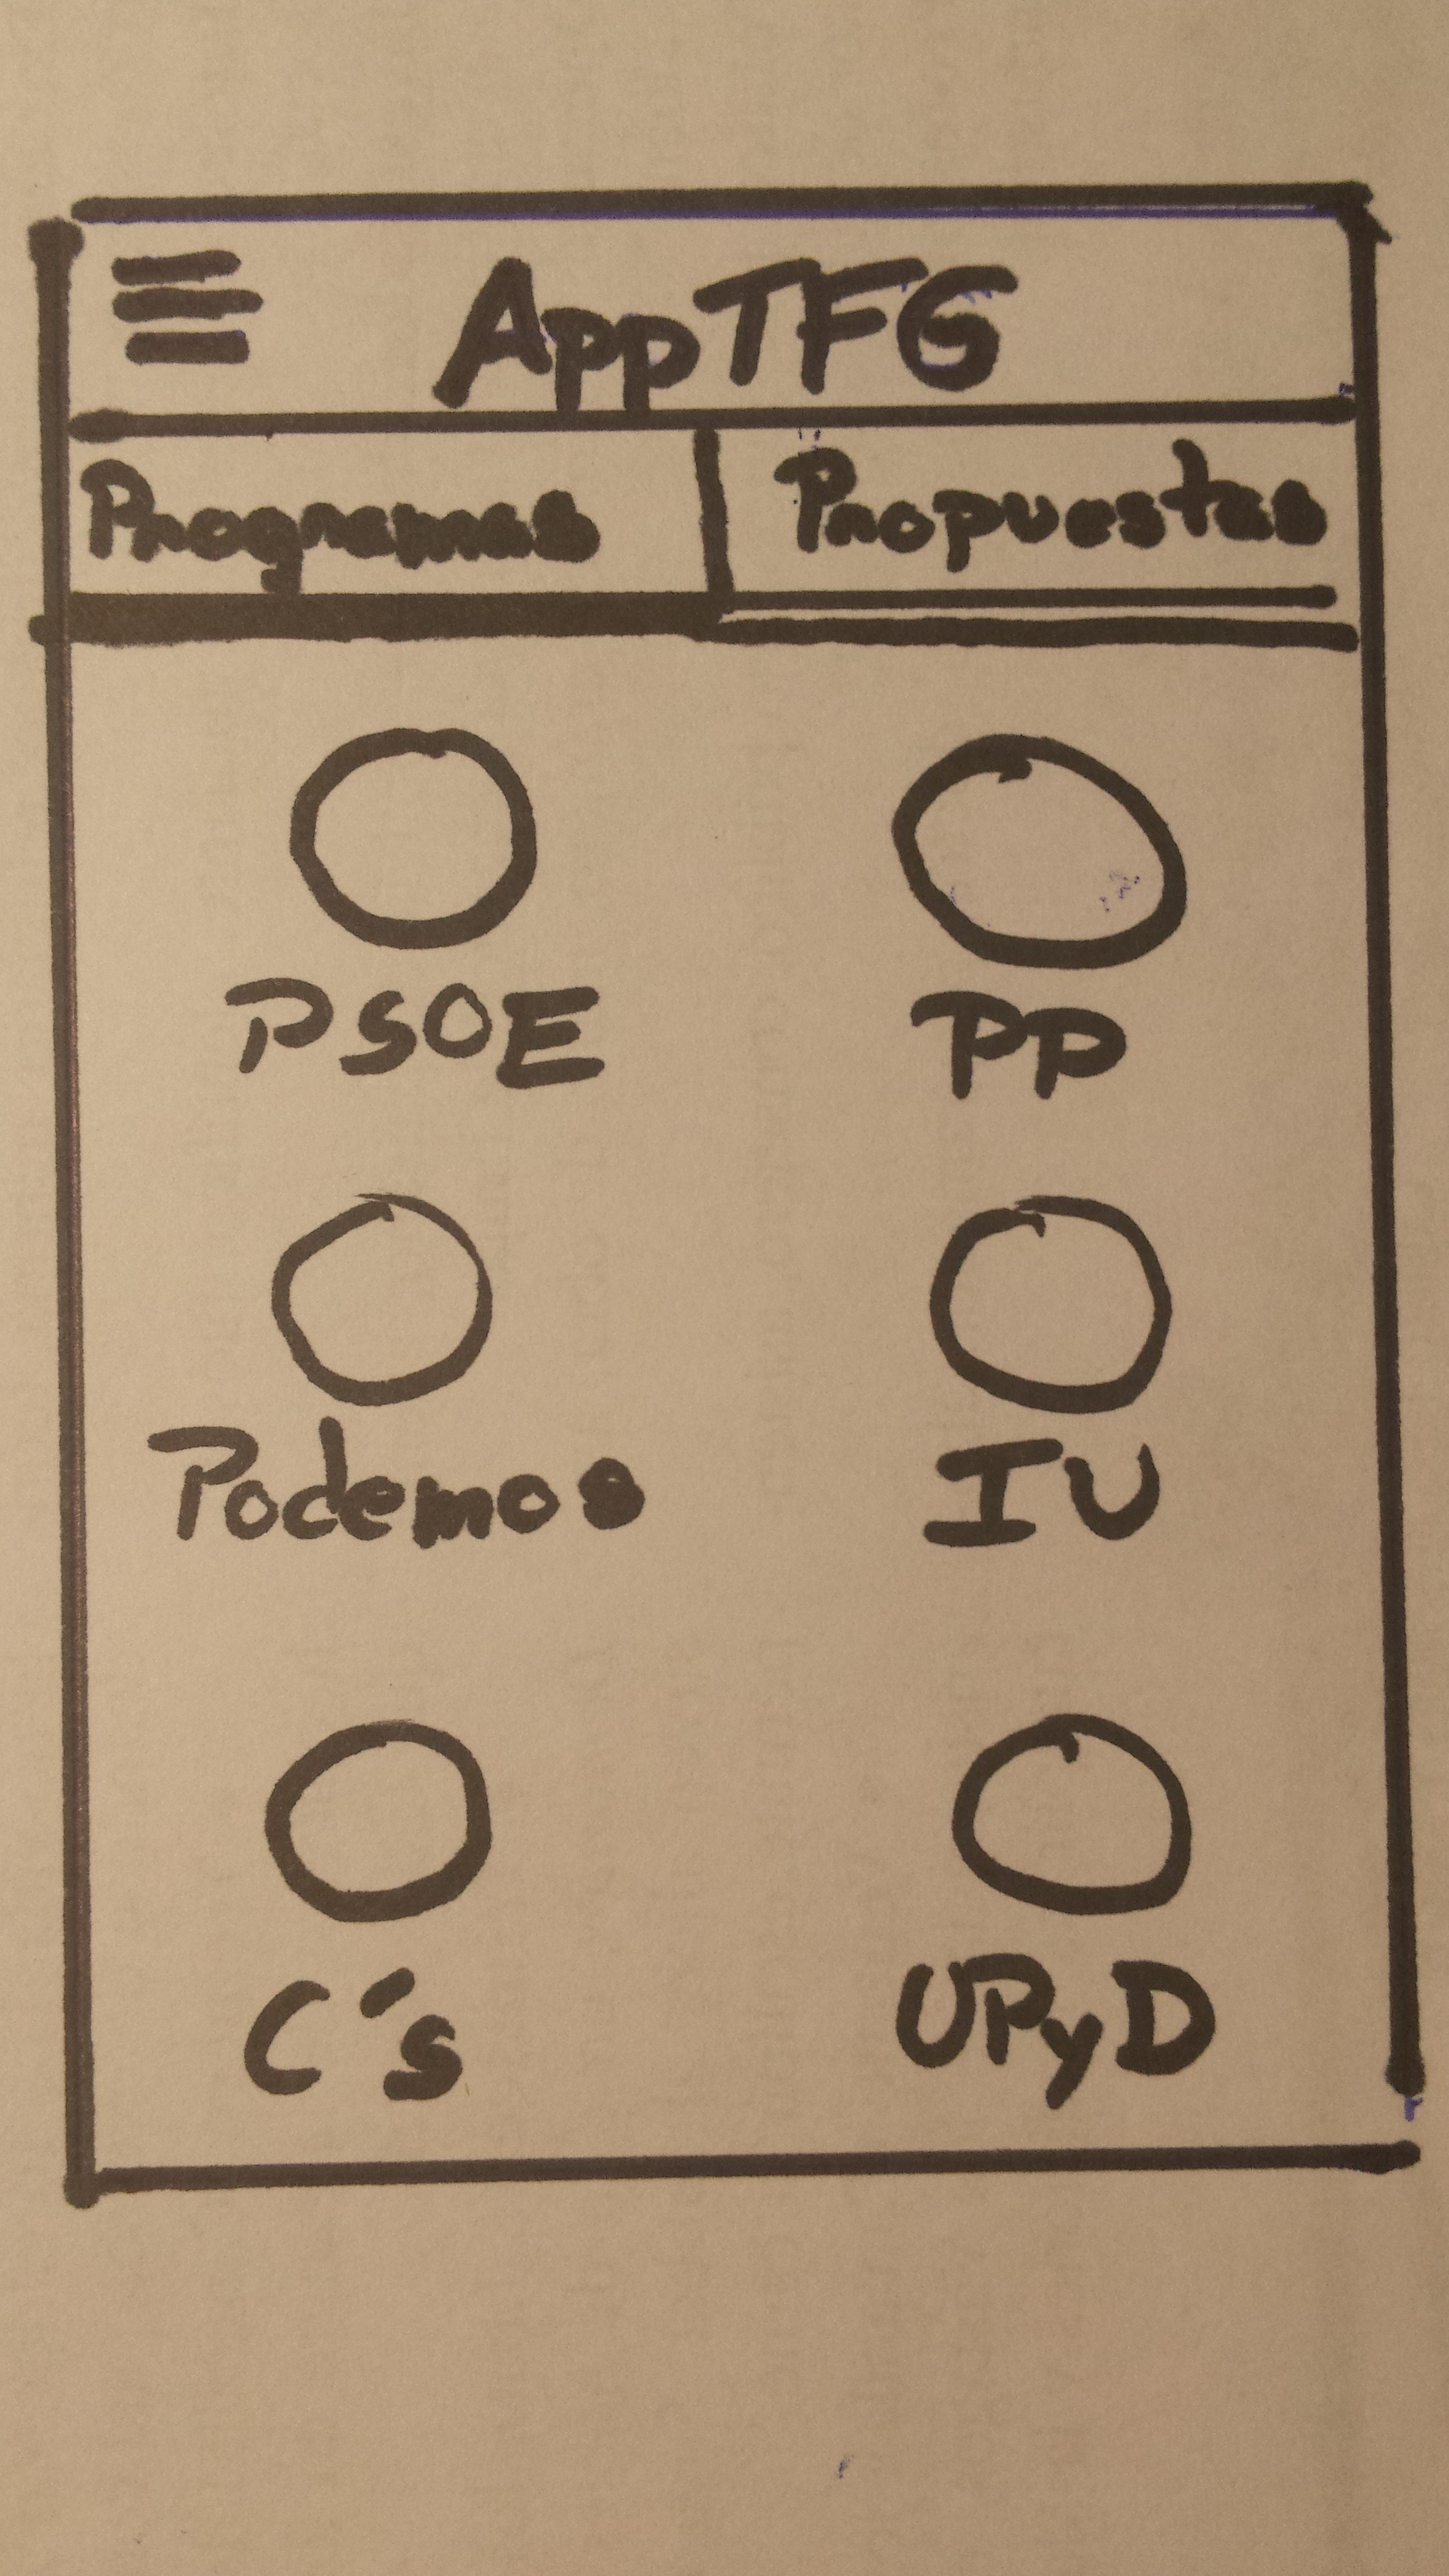
\includegraphics[width=\textwidth]{Media/Captures/prot1_1.png}
                \caption{Protipo en papel.}
                \label{fig:quipDesktop}
        \end{subfigure}
        ~
        \begin{subfigure}[b]{0.3\textwidth}
                \includegraphics[width=\textwidth]{Media/Captures/prot1_2.png}
                \caption{Protipo interactivo en POP.}
                \label{fig:quipText}
        \end{subfigure}
        ~
        \begin{subfigure}[b]{0.3\textwidth}
                \includegraphics[width=\textwidth]{Media/Captures/prot1_3.png}
                \caption{Implementación en Android.}
                \label{fig:quipComments}
        \end{subfigure}
        \caption{Primeros protitipos sobre programas electorales.}\label{fig:protPrograms}
	\end{figure}
	
\underline{Elementos del protitipo en papel}:

\begin{enumerate}
 \item Partidos políticos
 \item Programas políticos
 \item Índice de programas políticos
 \item Secciones de proramas políticos
\end{enumerate}

\underline{Funcionalidades del protitipo interactivo}:

\begin{enumerate}
 \item Visualizar la lista de partidos políticos.
 \item Seleccionar un programa político.
 \item Navegar por el índice de un programa polítco.
 \item Visualizar secciones de un programa, valorarla y comentarla.
\end{enumerate}

\underline{Implementación en Android}:

\begin{enumerate}
 \item Descargar la lista de partidos políticos del servidor.
 \item Descargar el programa seleccionado.
 \item Navegar por el índice del programa.
 \item Descargar el contenido de las secciones.
 \item Añadir comentarios al servidor.
 \item Modificar parámetros sociales en el servidor (like, dislike, views, etc).
\end{enumerate}

\item \textbf{Bocetos de Propuestas Ciudadanas}

A partir de lo desarrollado hasta el momento, se procedió a diseñar las propuestas en la aplicación. Manteniendo la coherencia con el diseño anterior, contuamos desarollando los protitipos que añadían la funcionalidad de las propuestas ciudadanas.

	\begin{figure}[H]
        \centering
        \begin{subfigure}[b]{0.3\textwidth}
                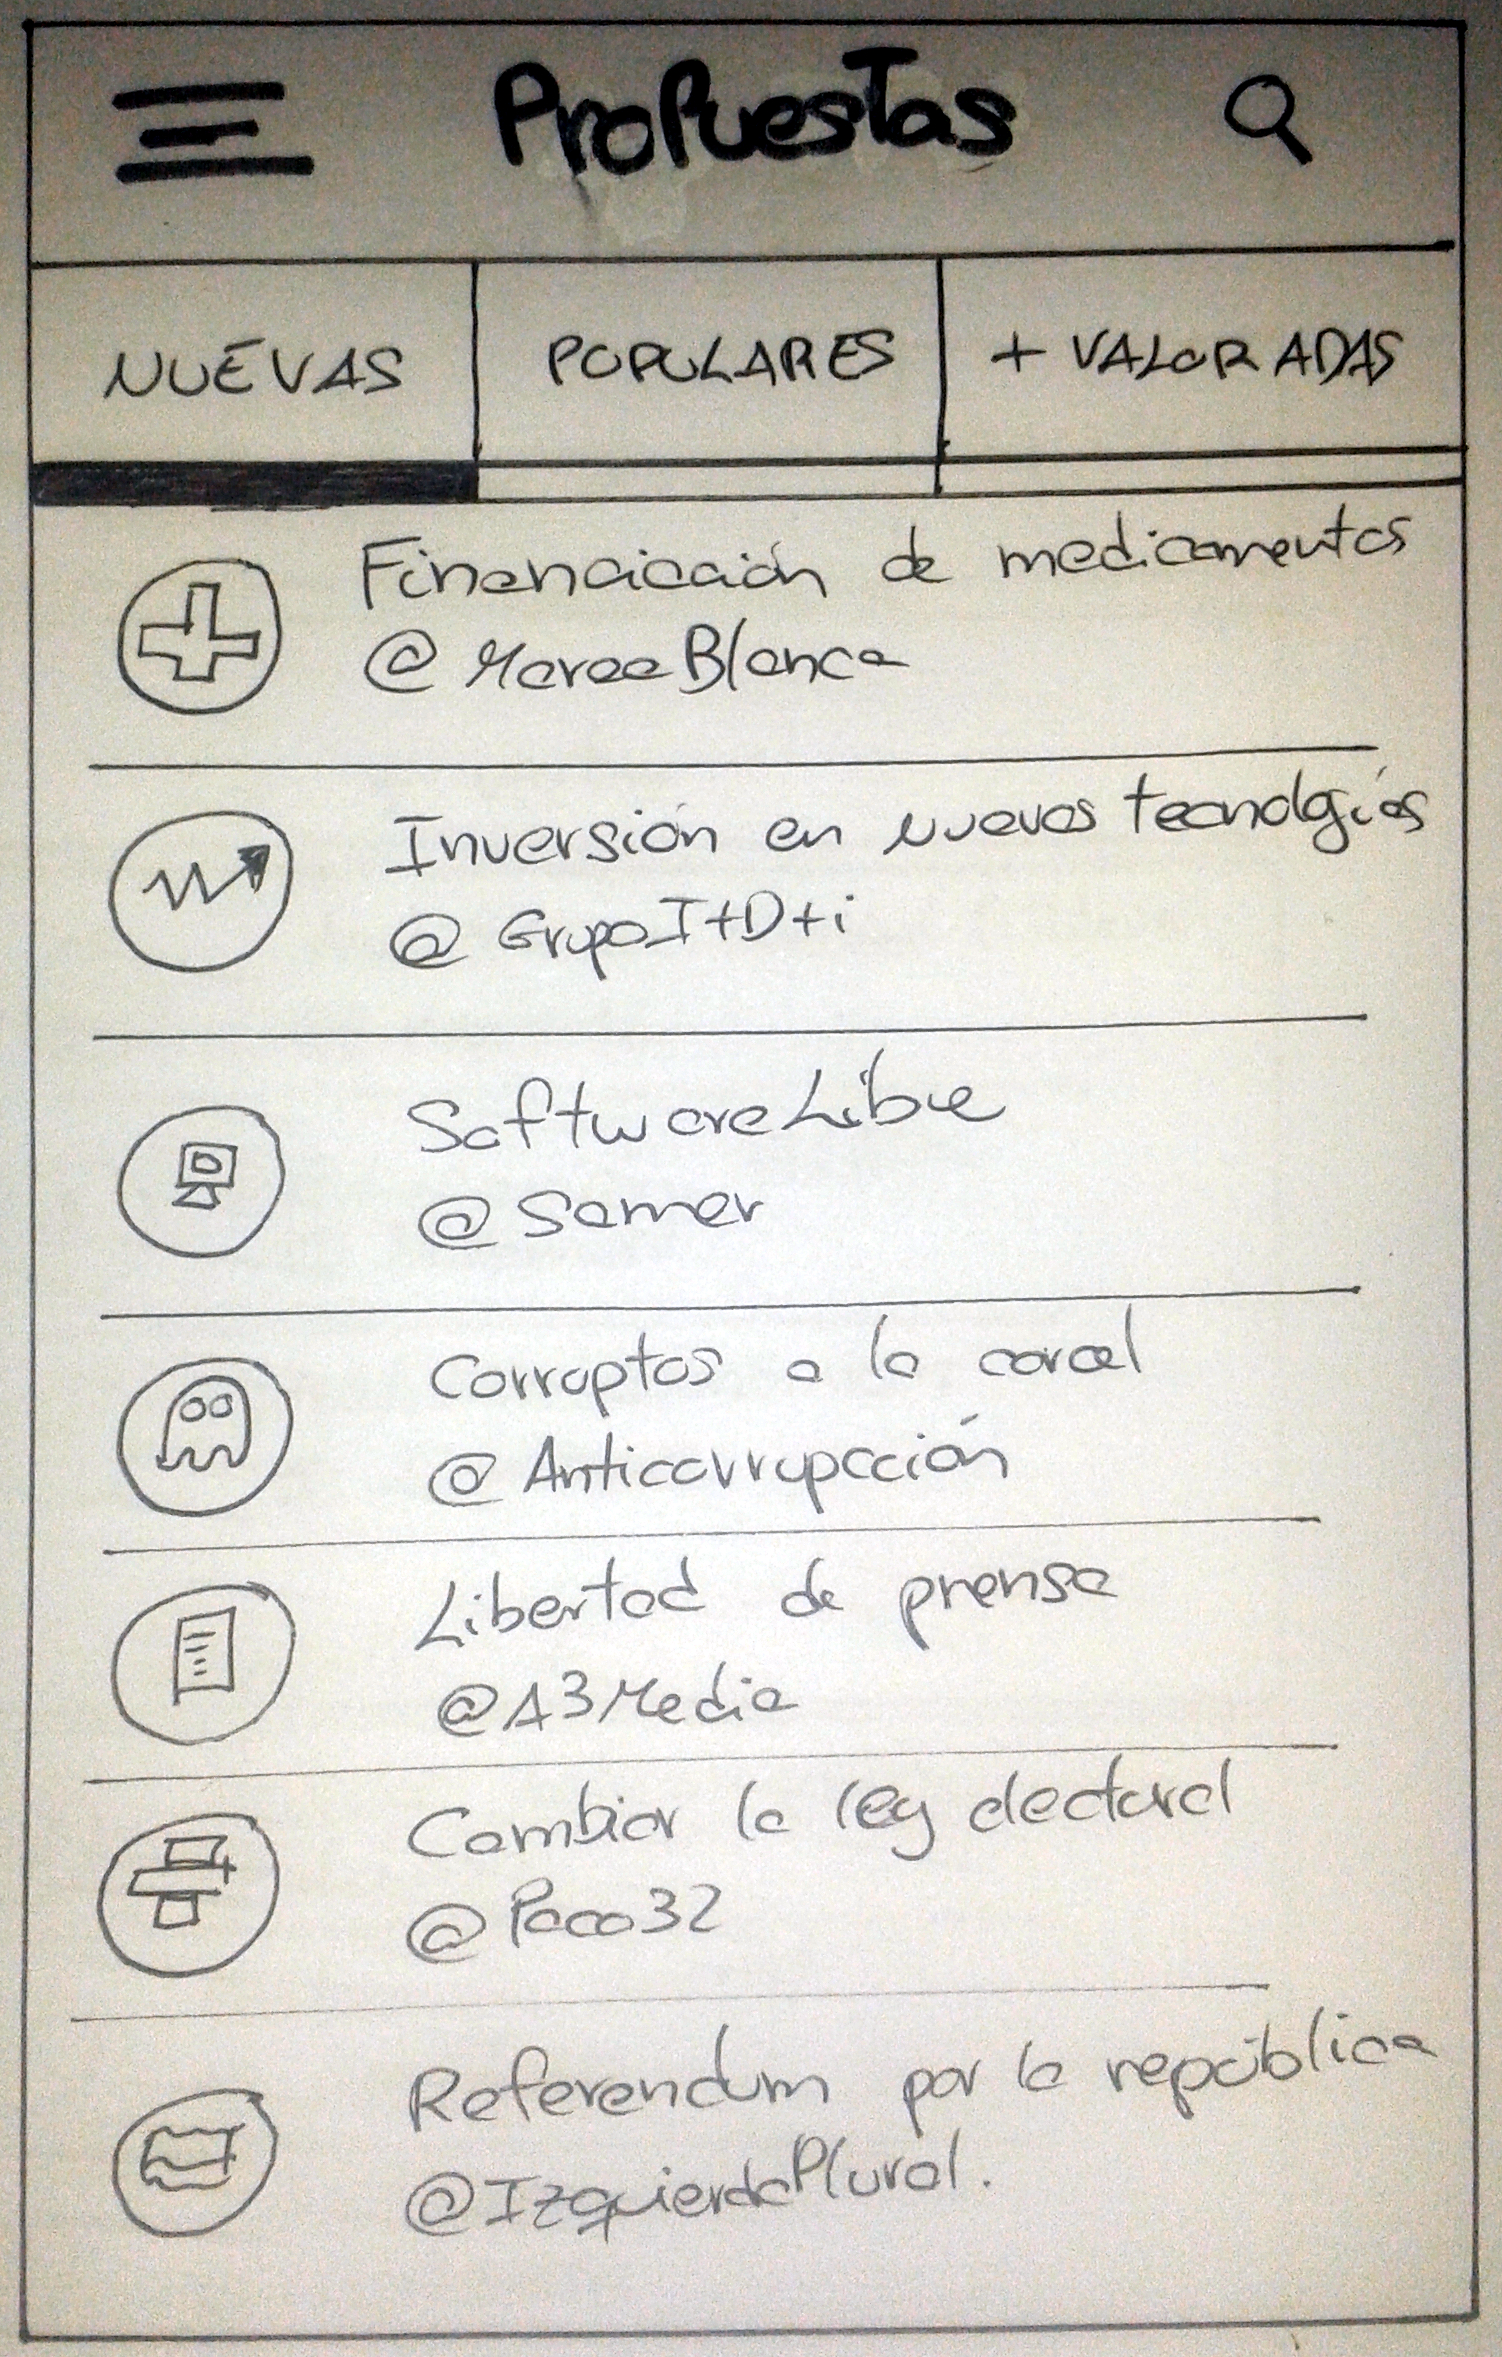
\includegraphics[width=\textwidth]{Media/Captures/prot2_1.jpg}
                \caption{Protipo en papel.}
                \label{fig:quipDesktop}
        \end{subfigure}
        ~
        \begin{subfigure}[b]{0.3\textwidth}
                \includegraphics[width=\textwidth]{Media/Captures/prot2_2.png}
                \caption{Protipo interactivo en POP.}
                \label{fig:quipText}
        \end{subfigure}
        ~
        \begin{subfigure}[b]{0.3\textwidth}
                \includegraphics[width=\textwidth]{Media/Captures/prot2_3.png}
                \caption{Implementación en Android.}
                \label{fig:quipComments}
        \end{subfigure}
        \caption{Prototipos para el desarrollo de propuestas.}\label{fig:protProposals}
	\end{figure}

\underline{Elementos del protipo en papel}:

\begin{enumerate}
 \item Propuestas ciudadanas.
 \item Listado de propuestas por tops.
 \item Listado de secciones de programas por tops.
 \item Desarrollar una propuesta.
 \item Pantalla principal rediseñada.
\end{enumerate}

\underline{Funcionalidades del prototipo interactivo con POP}:

\begin{enumerate}
 \item Visualizar propuesta.
 \item Listado de propuestas por tops.
 \item Listado de secciones de programas por tops.
 \item Desarrollar una propuesta.
 \item Pantalla principal rediseñada.
\end{enumerate}

\underline{Implementación en Android}:

\begin{enumerate}
 \item Visualizar propuesta almacenada en el servidor.
 \item Listado de propuestas por tops sincronizada con el servidor.
 \item Agregar una nueva propuesta al sistema.
 \item Pantalla principal rediseñada.
\end{enumerate}

\item \textbf{Bocetos de Propuestas Colaborativas}

\end{enumerate}

\textbf{Escenarios \textit{key path}}

En esta sección describiremos los escenarios \textit{key path}, que descrien cómo interactúa una persona con la interfaz diseñada en el framework de interacción. Son la evolución de los escenarios de contexto, pero describiendo cómo interactúa la persona con los elemenos de datos funcionales en la interfaz.

\begin{enumerate}[label=\textbf{\Roman*}]

\item \textbf{Escenario de cómo visualizar un programa político de un partido que se presenta a las elecciones.}

Faltan quince días para las elecciones generales y Carlos aún no ha decidido su voto. Un amigo le recomienda que instale \textit{DemoCritics} para poder leer algún programa político y ver las propuestas de las diferentes opciones políticas. Dentro de la aplicación, Carlos visualiza la lista de todos los partidos que se presentan a las próximas elecciones generales, y dentro de cada uno, puede visualiar el programa. Obteniendo un \textit{top} de las secciones más populares, Carlos visualiza las partes del programa que más llaman su atención.

\item \textbf{Escenario de cómo agregar una nueva propuesta en el sistema.}

Laura trabaja en la administración de la EMT y lleva varios días discutiendo con sus compañeros de trabajo una forma de reestructurar las líneas de autobuses. De forma que no confluyan todas en el centro, si no que alguna línea recorra los barrios exteriores del centro. Laura decide instalar \textit{DemoCritics} para poner en conocimiento de toda la ciudadanía la propuesta que lleva semanas trabajando. Para ello Larua se sitúa en la parte de \textit{propuestas} de la aplicación y agrega una nueva. Introduciendo la descripción de la propuesta, cómo piensa llevarla a cabo y el coste que supondría, Laura consigue publicar su propuesta en la aplicación para que los usuarios puedan valorarla y debatirla.

\item \textbf{Escenario sobre cómo solicitar ayuda para elaborar una propuesta.}

Manuel es un gran aficionado a la música, y en la localidad donde vive no hay escuelas de música municipales. Él quiere llevar a cabo una propuesta que se base en el desarrollo de nuevas escuelas de música municipales en puntos estratégicos y así fomentar la educación musical. Manuel toma su móvil en la pantalal principal de \textit{DemoCritics} y solicita la colaboración de una propuesta que facilite la creación de escuelas musicales. Ya que a pesar de ser un gran aficionado musical, Manuel no sabe cómo llevar a cabo esa propuesta o qué presupuesto necesitataría. Así pidiendo ayuda a los usuarios, Manuel tendrá desarrollada su propuesta por aquellos interesados y expertos del tema en la comunidad.

\item \textbf{Escenario para colaborar en el desarrollo de una propuesta.}

Sofía lleva varios años trabajando en la adminsitración pública del estado, y siempre ha querido ayudar utilizando la experiencia que le ha dado su trabajo estos años. Pero nunca ha sabido ni dónde ni cómo colaborar. Un conocido le recomienda instalar \textit{DemoCritics} en su móvil personal, así podría ayudar a personas que necesitaran ayuda de sus conocimientos. Con la aplicación instalada, Sofía se dirige a las propuestas colaborativas para explorar aquellas propuestas que están en desarrollo y pueden necesitar su ayuda. Seleccionada la propuesta, accede a su contenido y procede a editar el documento que explica cómo se llevaría a cabo la propuesta.

\end{enumerate}

\textbf{Escenarios de validación}

En esta fase se pondrán a prueba los escenarios, validando a ciertas situaciones que nos ayudarán a encontrar fallos o posibles mejoras en el diseño. Utilizaremos preguntas para definir la respuesta del sistema para problemas o dudas que puedan surgir.

\begin{enumerate}[label=\textbf{\Alph*}]

 \item \textbf{Qué pasaría si un usuario accede a la aplicación por primera vez y quisera consultar el programa político de un partido en concreto?}
 
 El usuario accedería a la pantalla principal de la aplicación (ver figura \ref{fig:mainFrameApp}), donde podría diferenciar cuatro grupos principales: \textit{Programas Políticos}, \textit{Categorías}, \textit{Propuestas Ciudadanas} y \textit{Propuestas Colaborativas}. Accediendo sobre el icono de programas políticos, la aplición mostraría al usuario el listado de partidos políticos para explorar los programas. Al usuario le bastaría con seleccionar el partido polítco del que quisiera consultar su programa electoral. Finalmente, la aplicación mostraría al usuario el índice del programa electoral del partido seleccionado. 
 
  	\begin{figure}[!]
      \centering
	\includegraphics[keepaspectratio, scale=0.2]{Media/Captures/mainFrame.jpg}
      \caption{Pantalla principal de la aplicación.}
      \label{fig:mainFrameApp}
    \end{figure} 
 
 \item \textbf{¿Cómo podría acceder un usuario a las secciones de todos los programas donde tratan un tema en concreto}
 
 Desde el menú principal, el usuario accedería al menú de \textit{categorías} para filtrar las secciones o propuestas por temas. Una vez allí, el usuario seleccionaría la categoría (ver figura \ref{fig:categoriesFrame}) que deseara para obtener todas las secciones de los programas de los partidos políticos que estuvieran relacionadas con esa categoría en concreto.
 
      	\begin{figure}[!]
      \centering
	\includegraphics[keepaspectratio, scale=0.3]{Media/Captures/categoriesFrame.png}
      \caption{Vista de categorías.}
      \label{fig:categoriesFrame}
    \end{figure} 
 
 \item \textbf{¿Qué tendría que hacer un usuario que queire publicar una nueva propuesta relacionada con la educación?}
 
 Debería ir al menú de \textit{propuestas} de la aplicación y seleccionar el botón de \textit{agregar} situado abajo a la derecha para acceder al formulario para publicar una nueva propuesta. Dentro del formulario, el usuario deberá de seleccionar la categioría de \textit{sanidad}
 
 \item \textbf{¿Cómo podría colaborar un experto en cultura en la aplicación?}
 
 Para ver si alguna propuesta requiere la ayuda de alguien en el mundo de la cultura, deberá acceder al menú \textit{Propuestas Colaborativas} y seleccionar la categoría \textit{Cultura} entre las listadas de la aplicación. Allí seleccionará aquellas propuestas que le resulten de interés para ayudar a su elaboración. Dentro de la propuesta podrá ayudar a redactar en un \textit{pad} colaborativo cómo llevar a cabo la propuesta o cómo financiarla.
 
\end{enumerate}

\subsection{Principios de Diseño}

Con el objetivo de verificar los principios de diseño que cumple la aplicación, utilizaremos los 10 principios de diseño propuestos por Jakob Nielsen \cite{ref:nielsen} para evaluar la calidad del sistema.

\begin{enumerate}
  \item \textbf{Visibilidad del estado del sistema}: Siempre que el sistema ejecuta tareas o no puede continuar por algún motivo, se mantiene informado al usuario sobre lo que está pasando. Esto podemos encontrarlo cuando el usuario accede a los programas políticos y el sistema procede a descargar la información. Mientras se descarga la información, se muestra un pequeño diálogo indicando la descarga de los datos para mantener al usuario informado.
  \item \textbf{Relación entre el sistema y el mundo real (Metáforas y lenguaje familiares)}: El sistema mantiene un lenguaje próximo al usuario, evitando terminos más formales del sistema. Cuando visualizamos una sección de un programa o una propuesta, el sistema emplea el lenguaje común de términos como \textit{like} (mano con pulgar hacia arriba), \textit{dislike} (mano con pulgar hacia abajo), etcétera, para valorar las secciones de un programa o una propuesta.
  \item \textbf{Control y libertad del usuario}: La aplicación permite deshacer acciones fácilmente, como puede ser cambiar la opinión de un \textit{like} o \textit{dislike}, o cancelar la acción de publicar una nueva propuesta o comentario.
  \item \textbf{Consistencia y estándares}: La aplicación sigue las pautas de diseño propuestas por las pautas de diseño \textit{Material Design} \cite{ref:materialdesign}. Este estilo de diseño plano fue propuesto por Google en 2014, y en la actualidad la mayor parte de aplicaciones móviles Android lo utilizan a la hora de diseñar sus pantallas. Por esto, los usuarios no deberían tener problemas navegando y utilizando los controles de la aplicación, ya que son familiare al encontrarse en un amplio catálogo de aplicaciones. Agregar una propuesta desde un botón de lapiz inferior situado a la derecha, representar un listado de objetos mediante \textit{tabs} deslizables, son algunas de las características destacables de \textit{Material Design}.
  \item \textbf{Prevención de errores}: La aplicación muestra mensajes de error cuando algo le impide funcionar con normalidad. De esta forma se avisa al usuario de que algo no está funcionando como debería. Cuando ejecutamos la aplicación y el sistema detecta que no hay conexión, la aplicación notifica al usuario en un sencillo diálogo la necesidad de tener conexión a internet para operar con la aplicacion.
  \item \textbf{Reconocimiento mejor que recuerdo}: Para agregar una nueva propuesta o comentario, tan sólo se necesita una transición entre dos pantallas. De esta forma facilitamos al usuario la generación de nuevos contenidos sin saturarle la memoria u obligarle a recordar mucha información para llegar a su objetivo. Este principio se encuentra en la mayor parte de las aplicaciones móviles, pues el usuario suele interactuar con el dispositivo en pequeños intervalos de tiempo y además no suele tener una postura cómoda que le facilite la concentración. Por lo que se requieren pocas transiciones entre pantallas, tareas sencillas y elementos sencillos y distinguibles. Por ejemplo, también identificamos las distintas partes de la aplicaión (Secciones, Categorías, Propuestas) con colores distintos para que el usuario sepa en todo momento dónde se encuentra.
  \item \textbf{Flexibilidad y eficiencia}: Se utilizan atajos a funcionalidades disponible desde la mayor parte de las pantallas del sistema. Haciendo uso del botón ''\textit{hamburguesa}'' en \textit{material design} nos da la posibilidad de abrir un menú con accesos directos a las principales partes de la aplicación. De tal forma que no necesitemos volver hacia atrás para seleccionar otra opción. No obstante, ambos caminos pueden ser utilizados en función de la habilidad o conocimiento del usuario respecto a la aplicación.
  \item \textbf{Estética y diseño minimalista}: Tanto los diálogos que muestra el sistema como la información visible en la mayoría de las pantallas del sistema es clara y concisa. Así evitamos dar información innecesaria al usuario o distraer su atención para evitar su confusión.
  \item \textbf{Ayudar a los usuarios a reconocer, diagnosticar y recuperarse de los errores}: Cuando el usuario da con un error inesperado, el sistema informa de lo ocurrido mendiante un sencillo diálogo de error. Simplificando el mensaje mostrado al usuario para que pueda resolverlo sin grandes problemas.
  \item \textbf{Ayuda y documentación}: Cuando el usuario genera contenido, el sistema  va indicando al usuario los pasos que tiene que seguir para completar su tarea de forma satisfactoria. Esto sucede por ejemplo en el caso en el que un usuario construye una nueva propuesta, donde el sistema le indica los campos que tiene que rellenar y la información que debe ir en cada campo.
\end{enumerate}

	\begin{figure}[!]
        \centering
        \begin{subfigure}[b]{0.3\textwidth}
                \includegraphics[width=\textwidth]{Media/Captures/principio01.png}
                \caption{Visibilidad del estado del sistema.}
                \label{fig:quipDesktop}
        \end{subfigure}
        ~
        \begin{subfigure}[b]{0.3\textwidth}
                \includegraphics[width=\textwidth]{Media/Captures/principio03.png}
                \caption{Control y libertad del usuario.}
                \label{fig:quipText}
        \end{subfigure}
        ~
        \begin{subfigure}[b]{0.3\textwidth}
                \includegraphics[width=\textwidth]{Media/Captures/principio07.png}
                \caption{Flexibilidad y eficiencia.}
                \label{fig:quipComments}
        \end{subfigure}
        \caption{Principios de diseño en la aplicación.}\label{fig:quipCaptures}
	\end{figure}